\subsection{Kortslutningssikring}
\label{effekt_kortslutningssikring}
Kortslutningssikringen tilføjes ved at indføre kredsløbet, vist på figur \ref{fig:dia-kortslut}, mellem base og emitter på darlingtontransistorerne, belastningen og tilbagekoblingen, som vist på figur \ref{fig:dia-kortslut1}. Her er dog kun vist for den halvdel af udgangstrinnet der er opbygget af en BDX33B, der skal dog indføres samme kredsløb på den halvdel der er opbygget af en BDX34B. 

\begin{figure}[h]
\centering
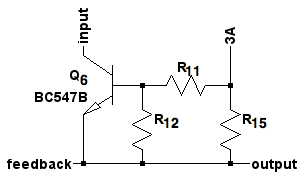
\includegraphics[scale=0.5]{teknisk/effektforstaerker/diagram-kortslut.png}
\caption{Overordnet diagram over kortslutningssikringens aktiveringssituation}
\label{fig:dia-kortslut}
\end{figure}

Strømmen på 3 A, anført på figur \ref{fig:dia-kortslut}, er den strøm, hvor kortslutningssikringen skal aktivere, hvilket blev bestemt i afsnit \ref{valg_kortslutningssikring}. At kortslutningssikringen skal aktivere betyder her, at transistoren Q1 skal åbnes. Når transistoren, Q1, åbnes vil den trække en strøm, hvormed strømmen ind i darlingtontransistorens base går mod nul og darlingtontransistoren lukker. 


\begin{figure}[h]
\centering
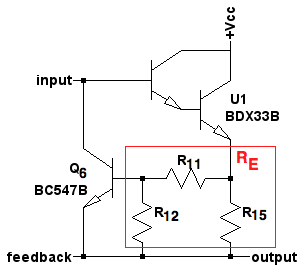
\includegraphics[scale=0.5]{teknisk/effektforstaerker/diagram-kortslut1.png}
\caption{Overordnet diagram over kortslutningssikring forbundet darlingtontransistor}
\label{fig:dia-kortslut1}
\end{figure}

Modstandene $R_1$, $R_2$ og $R_3$ skal, som vist på figur \ref{fig:dia-kortslut1}, repræsentere samme modstandsværdi som $R_E$, som blev beregnet i afsnit \ref{effekt_stroemforstaerker}, da den stadig skal sikre termisk stabilitet. For at åbne Q1 skal der, ifølge databladet for en BC547B \fixme{kilde: bc547.pdf}, være en base-emitter spænding på 720 mV, hvilket vil sige spændingen over $R_3$ skal være 720 mV når der løber 3 A fra darlingtontransistorens emitter. Dermed er det muligt at opstille de to udtryk vist formel (\ref{equ:kortslut-betingelse}) og i formel (\ref{equ:kortslut-betingelse1}) til bestemmelse af de tre modstande.

\begin{equation}
\label{equ:kortslut-betingelse}
\mathrm{536~m\ohm} = \frac{1}{\frac{1}{R_1}+\frac{1}{R_2 + R_3}}
\end{equation}

\begin{equation}
\label{equ:kortslut-betingelse1}
\mathrm{720~mV} = R_3 \cdot \frac{R_1 \cdot \mathrm{3~A}}{R_ 1+ R_2 + R_3}
\end{equation}

Det vides desuden, at modstanden af en parallelkobling af modstande er mindre end modstanden af den mindste gren i parallelkoblingen. Dermed vælges $R_1$ til den mindste tilgængelige effektmodstand som er større end den beregnede $R_E$. 

\subsubsection*{Simulering}